\documentclass[12pt]{article}
\usepackage{graphicx,amssymb}

\oddsidemargin  -0.5 cm
\evensidemargin 0.0 cm
\textwidth      6.5in
\headheight     0.0in
\topmargin      -1 cm
\textheight=9in

\renewcommand{\arraystretch}{1.25}

\title{Alignment of the CMS Muon System \\ with Tracks using a HIP-Based Algorithm}
\author{Jim Pivarski, Alexei Safonov, Karoly Banicz, Jim Bellinger, Riccardo Bellan}

\begin{document}
\maketitle

\section{Introduction and Motivation}

\begin{figure}
\begin{center} 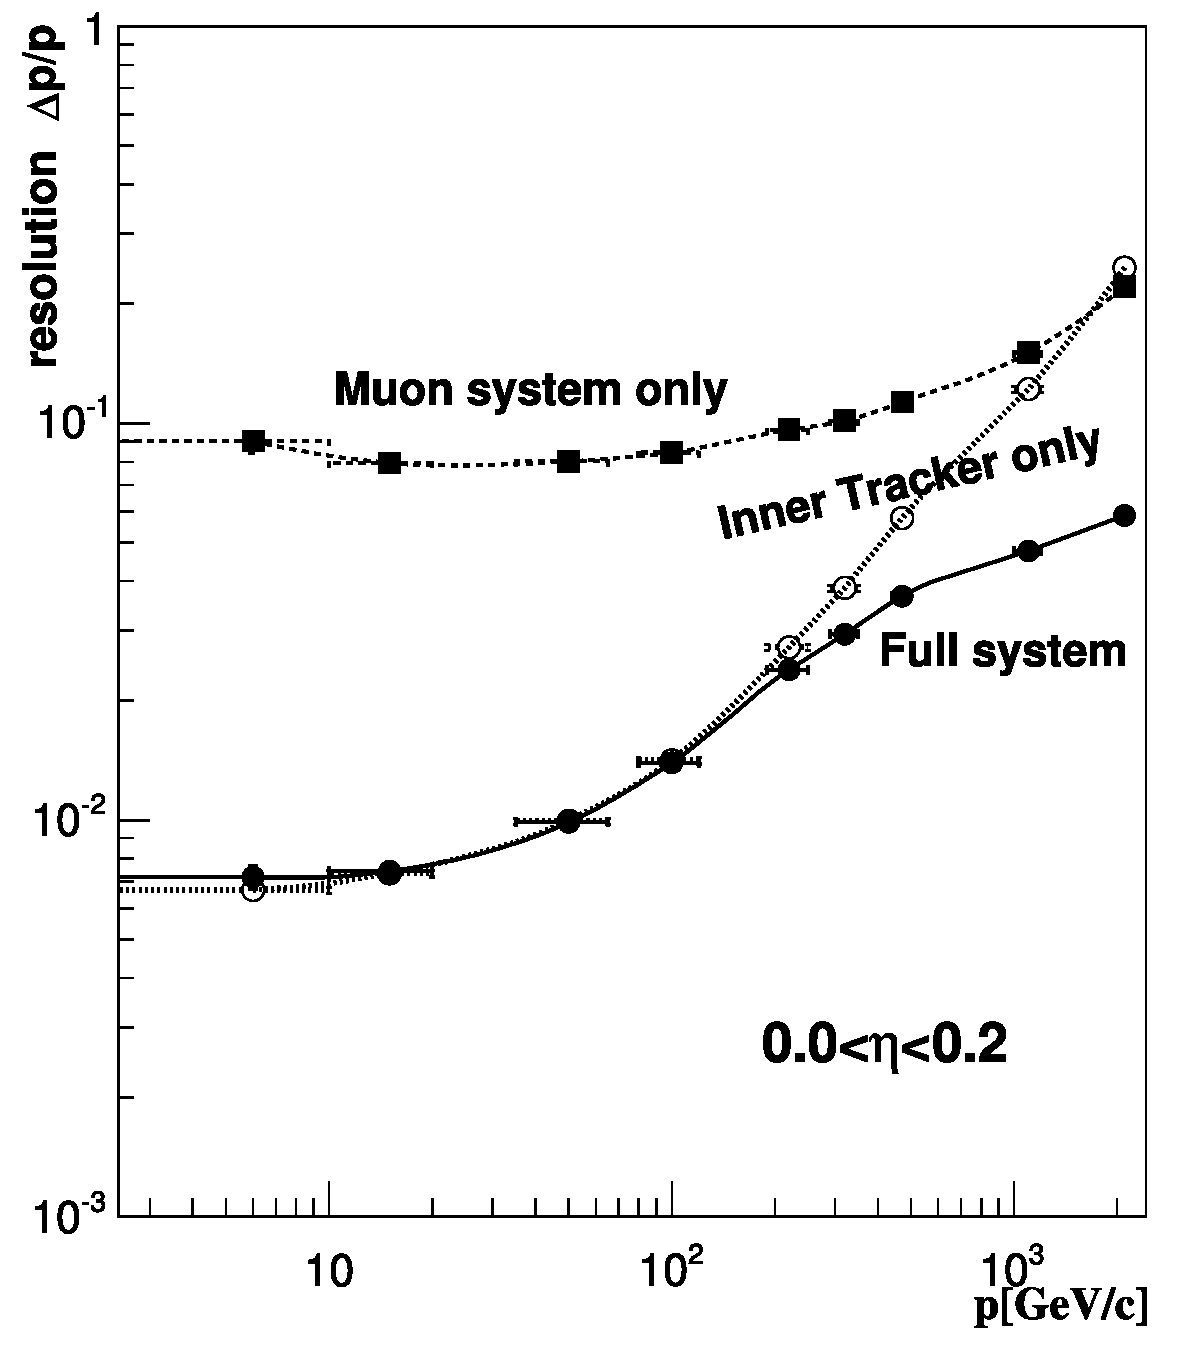
\includegraphics[width=0.45\linewidth]{Figure_001-005-a.png} 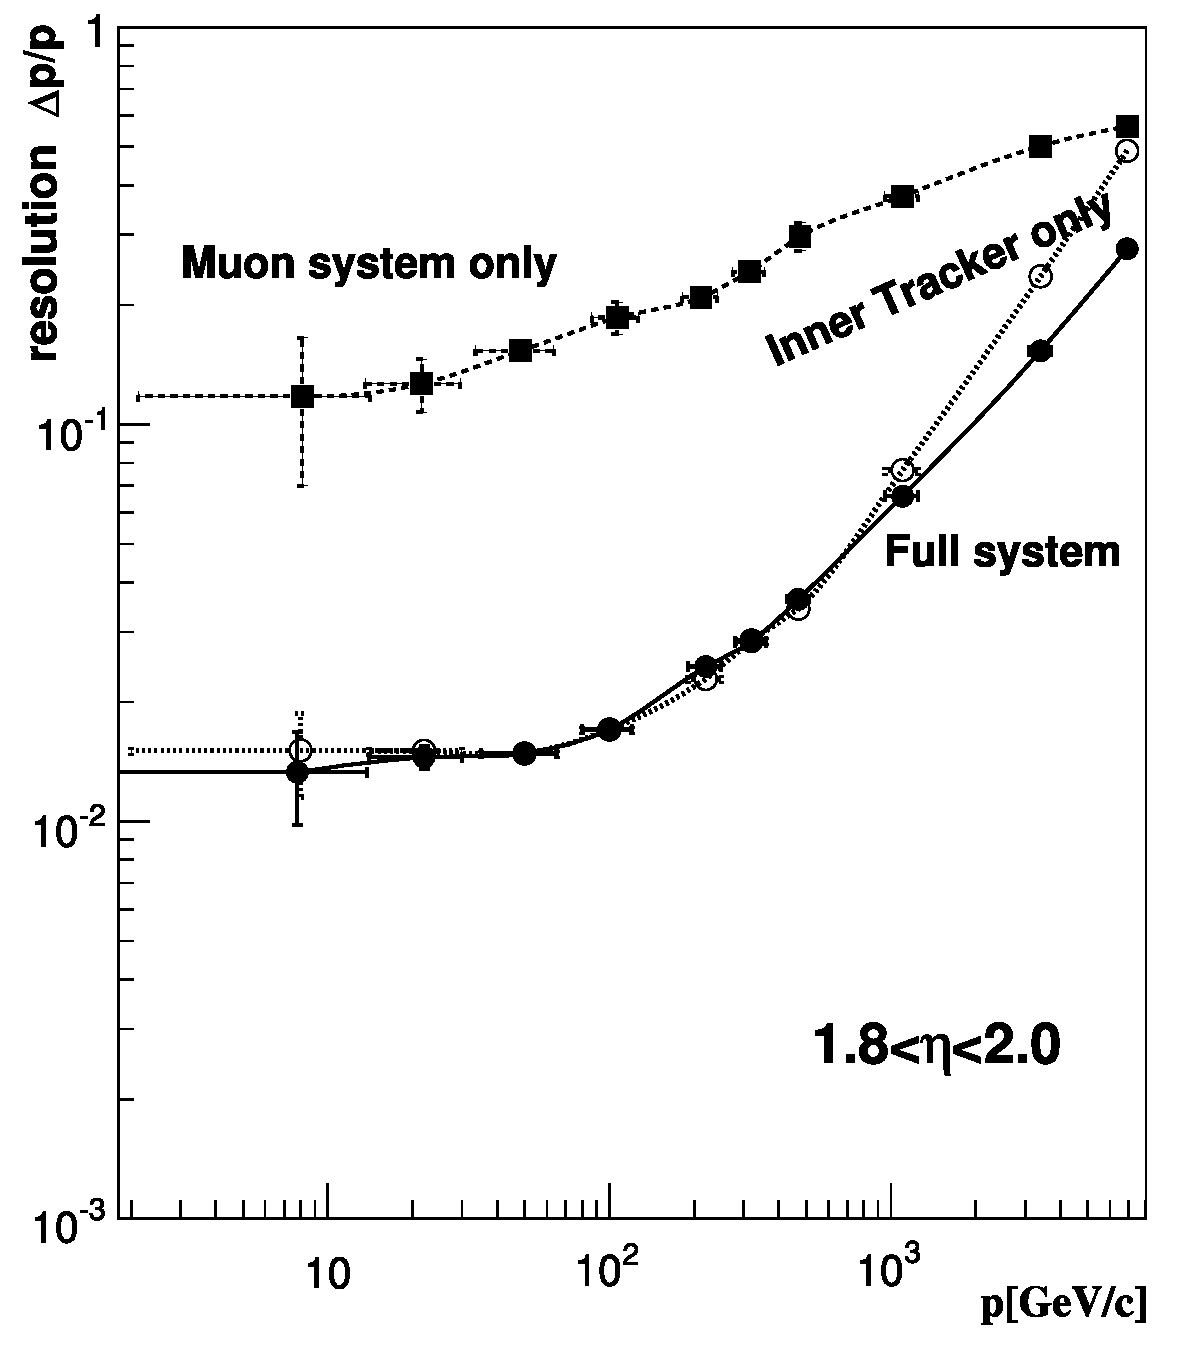
\includegraphics[width=0.45\linewidth]{Figure_001-005-b.png} \end{center}
\caption{Momentum resolution as a function of momentum.  The long
  lever arm of the muon system becomes a significant advantage for
  $p_T \gtrsim 200$~GeV, assuming that the muon chambers have been
  properly aligned. \label{fig:tdr_momentum_resolution}}
\end{figure}

show a $Z'$ plot, and say something brief about Heavy Stable Charged Particles

include statement on hardware alignment, how it relates with track-based

\section{Geometry of the Muon System and Coordinate Systems}

\begin{figure}
\begin{center} 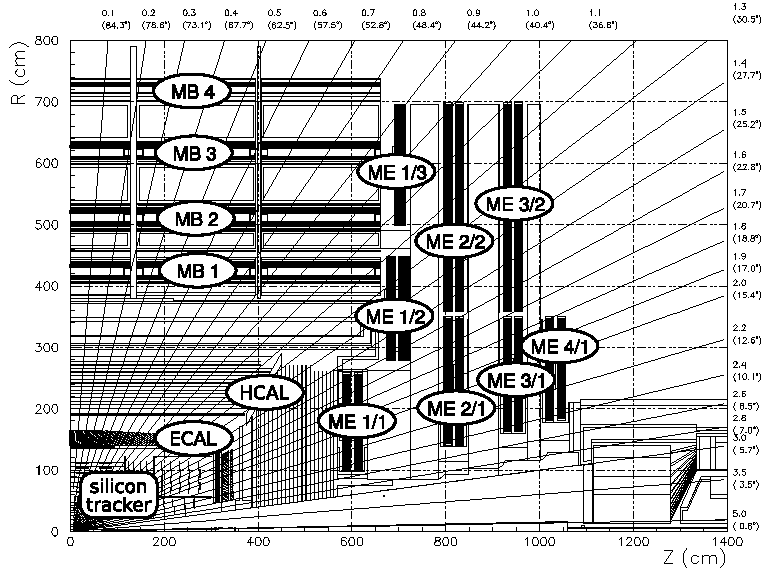
\includegraphics[width=\linewidth]{muon_system_labeled.pdf} \end{center}
\caption{A quarter-view of CMS, labelling the stations of the muon
  system.  ``MB'' and ``ME'' specify muon barrel and muon endcap,
  respectively.  The silicon tracker is inside $R < 120$~cm, $|z| <
  300$~cm \label{fig:muon_system_labeled}}
\end{figure}

define local $x$, $y$, $z$, $\phi_x$, $\phi_y$, $\phi_z$ for DT chambers, for CSC chambers

relate to global $r\phi$, $R$, and $z$

\section{Description of the Algorithm}

\begin{figure}
\begin{center} 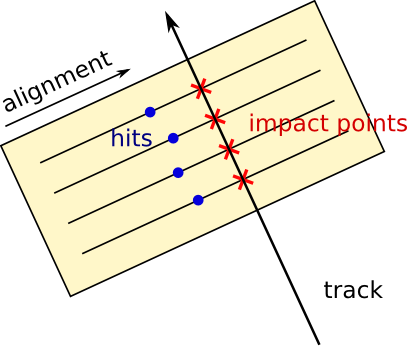
\includegraphics[width=0.35\linewidth]{hip_explanation.png} \end{center}
\caption{The alignment correction for each chamber is the offset of
  the peak of its residuals distribution from zero ($\mbox{residual}
  \equiv \left(\mbox{impact point}\right) - \left(\mbox{hit}\right)$).
  After alignment, the residuals are centered on
  zero. \label{fig:hip_explanation}}
\end{figure}

The HIP (``Hits and Impact Points'') algorithm accumulates residuals
distributions for each of the muon chambers, then adjusts the position
of each chamber by the offset of the peak of that distribution from
zero.  When tracks are refitted with the new geometry, residuals
should be centered on zero by definition.

A HIP algorithm is also used to align the silicon tracker, but the
HIP-based muon alignment algorithm has several important differences,
motivated by conditions in the muon system.  Each will be covered in
its own section below.

\subsection{Unbiased Residuals}
\label{sec:unbiased_residuals}

The globalMuon tracks used for alignment are refitted with normal
weights in the silicon tracker but artificially low weights in the
muon system (equivalent to an uncertainty-squared of 1000~cm$^2$),
such that the whole path of the refitted trajectory is determined
almost entirely by the tracker, yet muon residuals can still be
calculated in the normal way.  These residuals are unbiased in the
sense that the impact point is independent of the hit.

This technique is motivated by two facts about CMS:
\begin{itemize}
\item the uncertainty in the impact points of tracks propagated
  through the iron yoke and material in front of the first muon
  station is on the order of ???~mm due to random scattering in
  material, and
\item silicon tracker hits have a much higher intrinsic resolution
  than muon chamber hits (???~$\mu$m versus 100--300~$\mu$m in
  $r\phi$).
\end{itemize}

With normal weights, the track fitting algorithm would assume that a
large residual in the first hit of a muon chamber is due to scattering
in the material through which it propagated and pull the fitted
trajectory strongly to the hit.  Subsequent hits would have low
residuals that do not characterize the misalignment of the chamber.
By giving the muon hits low weights, the propagated trajectory instead
continues along the path of no scattering.  The resulting residuals
distributions are wider, but their peaks correspond more exactly to
the true misalignment of the chambers.

The second point above implies that this procedure does not lose
significant information.  Most alignment tracks have a $p_T$ well
below 50~GeV, so the muon system's long lever arm plays little role in
determining their curvature (Fig.~\ref{fig:tdr_momentum_resolution}).
Early tests of the procedure showed that the same alignment resolution
was reached by slowly converging with partly-biased residuals as by
determining the alignment in one step with unbiased residuals.

Unbiased residuals determine the alignment in one step because there
is no coupling between fitting the tracks and updating the muon
geometry.  The track parameters and full trajectories are independent
of the alignment, so the impact points in global coordinates are
largely unchanged when the procedure is repeated with a new geometry.
We perform a second iteration, but only as a verification step.  This
differs significantly from the tracker alignment procedures, in which
gradual convergence is an essential feature of the tracker-HIP
algorithm, and the tracker-MillePede algorithm solves a correlated
matrix of alignment parameters and track-fitting parameters.

The decoupling is possible because muon alignment is essentially a
different problem from alignment of the tracker, in which the shape of
the tracker must be determined in isolation.  The muon system must be
aligned in the same coordinate system as an external reference, the
tracker, and we can additionally take advantage of the high precision
of that reference to supply us with a fixed set of reference tracks.

\subsection{Residuals Peak-fitting Procedure}
\label{sec:residuals_peak_fitting}

Also as a consequence of large scattering, the residuals distributions
have non-Gaussian tails.  Residuals in the tails can pull the mean
away from its peak value, where the peak represents the true alignment
correction because high-quality tracks agree on the misalignment
measurement, and therefore the average residual, while poor-quality
tracks (scattering, measurement error) disagree in different ways and
don't form a coherent peak.  The effect is particularly significant if
the shape of the material in front of the muon chamber introduces an
asymmetry in this ``background'' distribution, or if the residuals
distribution has low statistics and is susceptible to being pulled by
a random sampling of tail events.

To account for the shape of the residuals distribution and to reduce
the weight that tail events have in determining the peak, we fit the
residuals to a physically-motivated distribution.  The fit is
unbinned, so there is a sense in which it is a small generalization of
simply calculating the mean.  The mean, $\sum_{i=1}^N r_i / N$, of a
set of residuals $\{r_i\}$ is equal to the peak $\mu$ of an unbinned
Gaussian fit $f(r_i, \mu, \sigma) =
\exp(-(r_i-\mu)^2/2/\sigma^2)/\sqrt{2\pi}/\sigma$.  What we do
differently is to make the fit function more realistic.  See
Sec.~\ref{sec:scattering_tails} for a complete description of the fit
function and fitting procedure.

The HIP procedure used to align the tracker determines the peak of
each residuals distribution through a weighted mean of residuals
(generalized to 6 alignment parameters).  The weighted mean reduces
sensitivity to scattering in the tracker case, but it would not be
effective in our muon alignment procedure because we de-weight the
muon hits uniformly in the track fit (see
Sec.~\ref{sec:unbiased_residuals}).

\subsection{Correlation of Hits}
\label{sec:correlation_of_hits}

The variance in unbiased residuals in a chamber on the same track is
much smaller than the variance in unbiased residuals in the chamber,
integrated over all tracks.  That is to say, the muon hits in a
chamber might be widely displaced from their associated track, but
they are all closely aligned with each other, because they correspond
to the physical path of a real muon, which may be offset from the
propagated track because of a scattering event somewhere along its
path.  Scattering events are unlikely to take place inside the muon
chamber because it is mostly a gas volume, and they are much more
likely in the iron layers between chambers.  The distribution of track
errors is also broadened by the fact that the tracks are
extrapolations from a distant silicon tracker.

To include all residuals indiscriminantly in a single peak-fit would
therefore underestimate the uncertainty in that fit.  In the limit of
zero intrinsic resolution, each track would encounter $N$ identical
residuals, where $N$ is the number of hits per chamber (6, 8, or 12,
assuming no inefficiencies).  A histogram of these residuals would be
an integral multiple of $N$ in every bin and a calculation of its mean
or a fit for its peak would have uncertainties underestimated by a
factor of $\sqrt{N}$.  If we instead average all the residuals on the
same track in the same chamber and put the result of that average into
the histogram, the uncertainties would be properly estimated.  (This
relies on the fact that the intrinsic resolution (100--300~$\mu$m) is
small compared to the distribution of track errors (few~mm).)

We can gain additional information by computing a linear fit to the
residuals as a function of local $z$ (layer number, accounting for the
layer spacings), weighted by intrinsic hit uncertainties.  The
constant term in this fit plays the same role as the average described
above, except that it always represents the hits-impact points
discrepancy at the center of the chamber (even with missing hits), the
point of the extended chamber body where alignment corrections are
applied.  The slope contains information about angular misalignment in
$\phi_y$ and $\phi_x$ (from $x$ and $y$ residuals, respectively).
This procedure is similar to calculating residuals with track
segments, rather than 1-dimensional hits, except that it only requires
the difference of the real and propagated tracks to be linear, not
each of them individually, and it benefits from any hit-pruning in the
reconstruction of the global track.

[We don't currently do this, though I expect to implement and test it
  in a matter of days.  The CRAFT constants were made with residuals
  weighted-averaged by chamber, but I want this Note to describe the
  finalized procedure, since we're close to a full implementation.
  The angular alignment from these slopes was an important feature of
  the CSC beam-halo alignment (in $\phi_y$).]

\subsection{Calculation of Alignment Parameters from Residuals}

An offset in the peak of local $x$ and local $y$ residuals from zero
clearly correspond to local $x$ and local $y$ translations, but the
relationship to local $z$ and angular alignment corrections is more
complicated.  There are many good ways to do this~[reference original
  HIP paper with Karimaki derivatives], and we have chosen an
especially practical and transparent approach.  Each parameter is
considered independently and computed from uncorrelated variables.

\subsubsection{Alignment Parameters for Muon Barrel Chambers}

DT chambers have two independent residuals distributions, local $x$
(corresponds to global $r\phi$) from superlayers~1 and 3 and local $y$
(corresponds to global $z$) from superlayer 2.  These 1-dimensional
hits are measured independently and are used for independent alignment
calculations.  Residuals on the same track in the same chamber are
combined in a weighted, linear, analytically-calculated fit, as
described in Sec.~\ref{sec:correlation_of_hits}.  The offsets and
slopes of these fits are accumulated into two independent residuals
distributions.  The peak of the ``offsets distribution'' is determined
by the fitting procedure described in
Sec.~\ref{sec:residuals_peak_fitting}: the deviation of this peak from
zero is the local $x$ or local $y$ alignment correction, depending on
whether it was computed from local $x$ or local $y$ residuals.  The
peak of the ``slopes distribution'' is determined via the same fitting
procedure, and its offset from zero is the $\phi_y$ or $\phi_x$
angular correction, depending on whether it was computed from local
$x$ or local $y$ slopes, respectively.

A slope in local $x$ residuals as a function of local $z$ corresponds
to a $\phi_y$ misalignment for the following reason: when a chamber is
rotated around the local $y$ axis, it introduces residuals in the
$x$-$z$ plane that grow linearly with distance from the rotation axis.
DT layers can sense $x$ residuals and their $z$ positions are known,
and the ratio $\Delta x/\Delta z$ is equal to $\tan \phi_y$ by
trigonometry (see Fig.~doesn't-exist-yet).  The angles are small, so
we neglect the tangent.  This derivation is exactly the same for
$\phi_x$ angles, swapping the roles of $x$ and $y$.

In principle, one could also look for $\phi_y$ and $\phi_x$ angles in
$x$ residuals vs.\ $x$ and $y$ residuals vs.\ $y$, respectively,
because the angular rotation would cause the chamber to appear to
become narrower.  However, this is a second-order effect in the angles
(Fig.~\ref{fig:phiy_explanation}) and a much less-sensitive way of
measuring the same thing.  [Maybe I shouldn't even have this paragraph
  and its associated Figure.]

\begin{figure}
\begin{center} 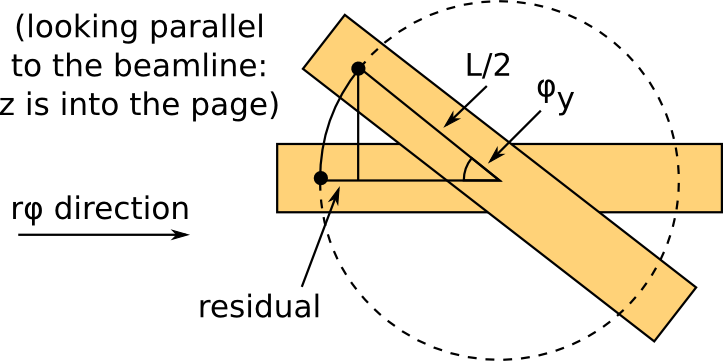
\includegraphics[width=0.35\linewidth]{phiy_explanation.png} \end{center}
\caption{This is way too small to see.  Well, maybe not after all the other, larger, effects have been taken care of first. \label{fig:phiy_explanation}}
\end{figure}

The third angle, $\phi_z$ doesn't rotate segments, but it does
introduce a linear trend in local $x$ residuals as a function of local
$y$ and local $y$ residuals as a function of local $x$.  Because DT
chambers are longer in the $y$ dimension than the $x$ and also because
$x$ residuals are more precise, the local $x$ residual vs.\ $y$ trend
is the most precise way to measure the angle.  We split local $x$
derivatives into two bins: one with $y<0$ and the other with $y>0$,
and compute the peak positions from the ``offsets distributions'' in
each of these independently.  The average of the two bins' results is
the local $x$ alignment [a minor modification of what was written
  above], and the difference of the two bins is used to calculate
$\phi_z$.  Specifically,
\begin{equation}
\phi_z = \frac{\mbox{$x$ residuals peak in $y<0$ bin} - \mbox{$x$ residuals peak in $y>0$ bin}}{\mbox{average $y$ of $y<0$ bin} - \mbox{average $y$ of $y>0$ bin}} \mbox{.}
\end{equation}
As a cross-check, we observe $y$ residuals vs.\ $x$ in our validation
plots, to make sure it is also corrected by $\phi_z$ alignments
computed from $x$ residuals vs.\ $y$.

Thus we align $x$, $y$, $\phi_x$, $\phi_y$, and $\phi_z$ using
quantities which are not only linearly independent of one another, but
orthogonal.  There are no correlations between them that would require
iteration.

[Local $z$ is special.  We need to align the other parameters first,
  and then possibly iterate with this one.  It is not the case that we
  are insensitive to it; we are sensitive in $x$ residuals vs.\ $x$
  and $y$ residuals vs.\ $y$, but only to the degree that the tracks
  come from a point source.  In other words, this is a great
  collisions-muons measurement, more difficult with cosmic rays.]

\subsubsection{Alignment Parameters for Endcap Chambers}

Treat CSCs as 1-dimensional residuals (that is, ignore wires), but use
the fact that strip measurements are a linear combination of $x$ and
$y$, and that combination varies over the width of the chamber.  $y$
will be less sensitive than $x$ this way, but that's all right.  Then
when we have $x$ and $y$, we can do all the same tricks as with the
DTs.  We'll just need to be careful how we organize bins, so that
measurements remain uncorrelated.

\subsection{Validation Techniques}

those plots I've been making

\section{Controlling for Systematic Effects}

\subsection{Tails in Residuals from Scattering Processes}
\label{sec:scattering_tails}

\subsection{Momentum-Dependent Residuals from Magnetic Field and Material Budget Errors}

The two bins in $q/p_T$ quantifies errors from both a wrong
$\vec{B}$-field and a wrong $dE/dx$.  The former is linear in $q/p_T$,
and the latter is very nearly an antisymmetric parabola ($x^3/|x|$).
They are both antisymmetric, which makes this safer than a linear fit
to the distribution.

[We need to add a cut to reject high $p_T$ events, because charge
  confusion at high momenta with a non-unit charge ratio makes the
  two-bin cancellation imperfect.  The cut will be about $p_T <
  100$~GeV, which is already nearly applied by the cosmics
  distribution itself.]

\subsection{Systematic Errors from Imperfect Tracker Alignment}

\subsection{Non-uniform illumination}

dividing the chamber up into four parts, taking averages; works as
long as the distribution of illumination is linear

\section{Validation Plots and CRAFT Cosmic Ray Results}

\section{Simulated Alignment with Collisions}

With the up-to-date Summmer08 samples, we can quickly run the
finalized procedure on the equivalent of 50~pb$^{-1}$ of inclusive
single-muon, and perhaps as much $W^\pm$ and $Z$, thus producing a
much more relevant version of the CSA08 study.  There will be a new
tracker STARTUP scenario (using what they learned from CRAFT) that we
can use to quantify dependence on the tracker.

\section{Alignment Tools in CMSSW}

\begin{itemize}
\item Alignment algorithm: \\ {\tt Alignment/MuonAlignmentAlgorithms/plugins/MuonAlignmentFromReference}
\item Track refitter: \\ {\tt TrackingTools/TrackRefitter/plugins/TracksToTrajectories}
\item Database comparison and modification tool: \\ {\tt Alignment/MuonAlignment/plugins/MuonGeometryDBConverter} \\ with full documentation at \\ {\tt https://twiki.cern.ch/twiki/bin/view/CMS/SWGuideMuonGeometryConversion}
\item Database comparison plots for local differences: \\ {\tt Alignment/MuonAlignment/plugins/MuonGeometryArrange}
\item Track-based validation: \\ {\tt Alignment/CommonAlignmentMonitor/plugins/AlignmentMonitorMuonGeometryMap} [not in CVS yet]
\end{itemize}

\section{Conclusions}

\section{References}

\end{document}
